% http://www.idsc.ethz.ch/education/theses-semester-projects.html
% IDSC LaTeX Thesis Template
% 
% Author(s):	Eric Müller
% 				Institute for Dynamic Systems and Control
% 				Swiss Federal Institute of Technology (ETH) Zurich
% 
% Created:		2004/04/02  (Eric Mueller)
% 
% Notes: Has been tested on Windows 7 + MikTeX + TeXnicCenter
%
% Revisions: 	2009/05/29  (Soren Ebbesen)
% 				    2011/03/22	(Soren Ebbesen)
%             2013/03/08	(Soren Ebbesen)
%             2014/03/13	(Soren Ebbesen)
% ______________________________________________________________________________
\documentclass[12pt,oneside,a4paper,fleqn]{article}
\usepackage{siunitx}
%\usepackage[utf8]{inputenc}
\usepackage[onehalfspacing]{setspace}
%\usepackage{lineno}\linenumbers

% CHANGE HERE FOR GERMAN (german) OR MASTER THESIS (mt)!!!!!

\usepackage[english,bt]{ethidsc} % Special IDSC styles and commands      	
								 % {german}/english: language of headings, etc.
								 % {st}/bt/mt: {semester}/bachelor/master thes
\addbibresource{references.bib}
\usepackage{calligra}
\usepackage{mathtools}
\usepackage{amsmath}
\usepackage{float}
\usepackage{siunitx} 
\usepackage{array}
\usepackage{hyperref}
\usepackage{graphicx}
\usepackage{booktabs}
\usepackage{geometry}
\usepackage{subcaption}
\usepackage{amssymb}
\usepackage{microtype}
\usepackage{braket}
\usepackage{cleveref}

% Page header (don't change)____________________________________________________
\setlength{\parindent}{0em}                 % Disable parindent
\rhead[\nouppercase{\rightmark}]{\thepage}  % Special headings
\lhead[\thepage]{\nouppercase{\leftmark}}   % Special headings
\cfoot{}                                    % Special headings


% Title page (please fill in)___________________________________________________
\title{Influence of probabilistic abstention on spatial cooperative games}


\studentA{Alessandro Azzani, Francesco Gargiulo \\ Lea Haas}
%\ethidA{20-000-00}
%\semesterA{6}
%\emailA{someone@student.ethz.ch}

\studentB{Nicol\`{o} Montalti}
%\ethidB{12-345-678}
%\semesterB{9}
%\emailB{second@student.ethz.ch}

%\supervision{Prof. Dr. Superviser}
\date{\today}

%\identification{IDSC-XX-YY-ZZ} 		% Project identifier

%\infopage
%\declaration

% Begin document________________________________________________________________
\begin{document}

\maketitle 							% Create title page

\pagenumbering{roman}
\tableofcontents
\newpage
% Preamble______________________________________________________________________

%\pagenumbering{roman} 				% Begin roman page numbering (i,ii,...)

%\input{chapters/preamble} %Abstract etc.

% Chapters______________________________________________________________________

\pagestyle{fancy}               	% Fancy headings			
\setlength{\parindent}{20pt}

% We start writing from here -----------------------------------------------------
\addcontentsline{toc}{section}{Individual contributions}
\section*{Individual Contributions}
\label{chap:indv}

Who did what....

\newpage
\addcontentsline{toc}{section}{Introduction}
\section*{Introduction}
\label{chap:intro}
\pagenumbering{arabic}


Here we write the introduction


\section{Theoretical background}
In this section, we want to elaborate on the theoretical background of the project.
\subsection{Games}
%PD, SH, HG, SD
%sd also called chicken/ hawk dove
%different strategies and cooperation vs defection
%\cite{nowak_sigmund_2000} for the 4 games

\subsection{Evolutionary Game theory}
%makes the system more dynamical, allow for various app

\subsection{Spatial games}
% repeated games, imitation, noise
%\cite{nowak_may_1992}: fist time they did evolutionary game theory on a grid


\subsection{Abstention}
% optional abstention, probabilistic abtention (PD, OPD, PDPA)
% (paper: DOI:10.1038/s41598-018-32933-x)


\section{Implementation}
The game has been implemented in Python, the code is publicly available on GitHub \cite{montalti2023}.
The spatial environment has been implemented as a $50 \times 50$ 2-dimensional grid.
A player is present at every point of grid.
Every player is characterized by a strategy (collaborate or defect) and by an abstention probability $\alpha \in [0,1]$.
The game is defined by the five parameters $T, R,  P, S, L$ and by a noise factor $\eta \in [0,1]$.
The first five parameters determine the game played: prisoner dilemma (PD), snowdrift (SD), stag hunt (SH) or harmony game (HG).

The game is initialized assigning to each player a random strategy, with a $50-50$ probability, and an abstention probability $\alpha$. The latter can be assigned in three different ways:
\begin{itemize}
    \item No abstention: $\alpha = 0$ for all players. The game is reduced to the standard prisoner dilemma (PD) or another standard game;
    \item Optional abstention: $\alpha = 0$ or $1$ with a $50-50$ probability. The game is reduced to the optional prisoner dilemma (OPD) or the equivalent for another game;
    \item Probabilistic abstention: $\alpha \in [0,1]$. The players have a finite probability of abstention, distributed between 0 and 1 with steps of 0.125. In particualr, the values that it can assume are
    $\alpha = \{0, 0.125, 0.25, 0.375, 0.5, 0.625, 0.750, 0.875, 1 \}$.
    We call this situation prisoner's dilemma with probabilistic abstention (PDPA) or the equivalent for other games.
\end{itemize}

At each iteration of the game, each player plays against their four nearest neighbours.
Each player earns an amount equal to the sum of the payoff of the four games they played with the neighbours.
The payoff of a single match between two players is determined by the game played, the strategy of the two players and by their abstention probability.
Each player joins the game with a probability $1-\alpha$.
If both players join the game, the game is played and payoffs are distributed according to the players strategies.
If one of the players abstains, the game is not played, and both players receive a payoff $L$.

After every player has played, the imitation process begins.
The imitation process is influenced by the noise parameter $\eta$.
In particular, each player randomly changes their strategy to the opposite strategy with a probability $\eta$ and imitates rationally their best performing neighbours with a probability $1-\eta$.
If the imitation option is chosen, the player looks at their four nearest neighbours payoffs, and imitates the strategy of the one who performed the best in the last round.
If more players share the same optimal outcome, a random one is chosen.
In addition to imitating the best-performing player's strategy, the abstention probability of the most performing neighbour is imitated as well.

The process is iterated for a fixed number of times $t$ (usually $t=200$).
At each iteration, the players play the game and imitate their neighbours' strategies and abstention probabilities.
At the end of the cycle, some statistics are extracted from the final configuration.
Taking inspiration from Cardinot \emph{et al.} \cite{cardinot2018}, we evaluate the mean abstention probability $\langle \alpha \rangle$ and the mean effective cooperation frequency $\varepsilon = (1-\alpha)\cdot (1-s)$, where $s = 0$ for a cooperator and $s=1$ for a defector.
In addition to these two quantities, we also analyse the correlation between being a cooperator and having a low abstention frequency $\alpha$. 
To do so, when playing the version of the game with probabilistic abstention, we plot the number of cooperators and defectors for each value of $\alpha$ at the end of the cycle and compare the results.


\section{Results}
\label{sec:results}

First of all, we start by comparing our results with the ones obtained by Cardinot \emph{et al.} \cite{cardinot2018} for the dependence of the effective cooperation frequency $\varepsilon$ and of the mean abstention probability $\alpha$ on the temptation payoff $T$ in the prisoner's dilemma game.
This comparison is shown in \Cref{fig: comparison of epsilon and alpha}.

\begin{figure}[H]
    \centering
    \subfloat[]{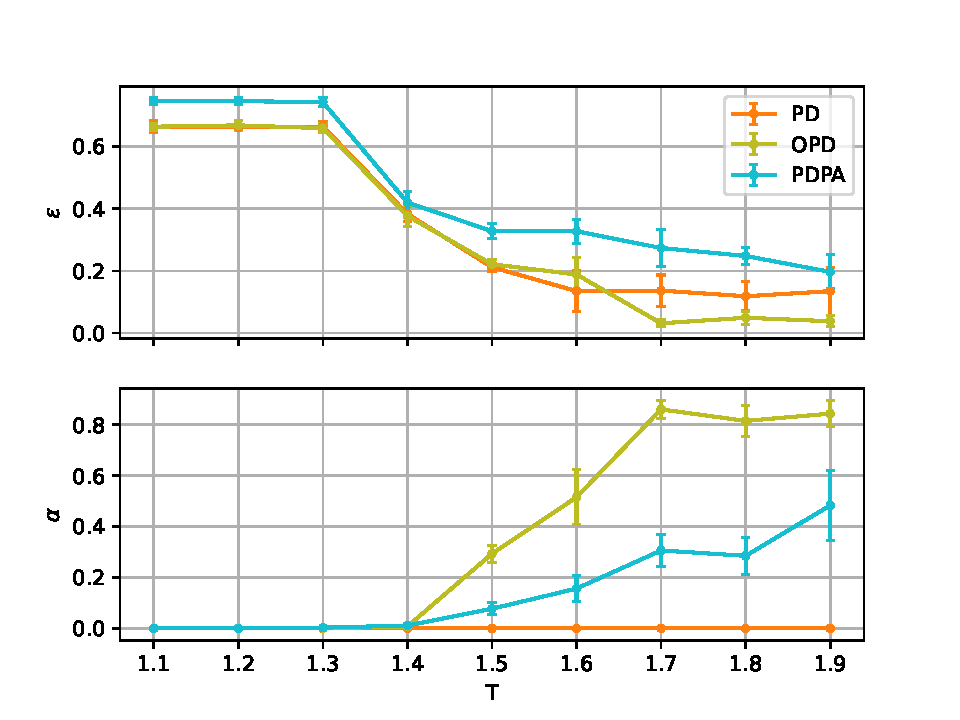
\includegraphics[scale = 0.5]{Images/alpha_eps-20230606-125503.pdf}}
    \subfloat[]{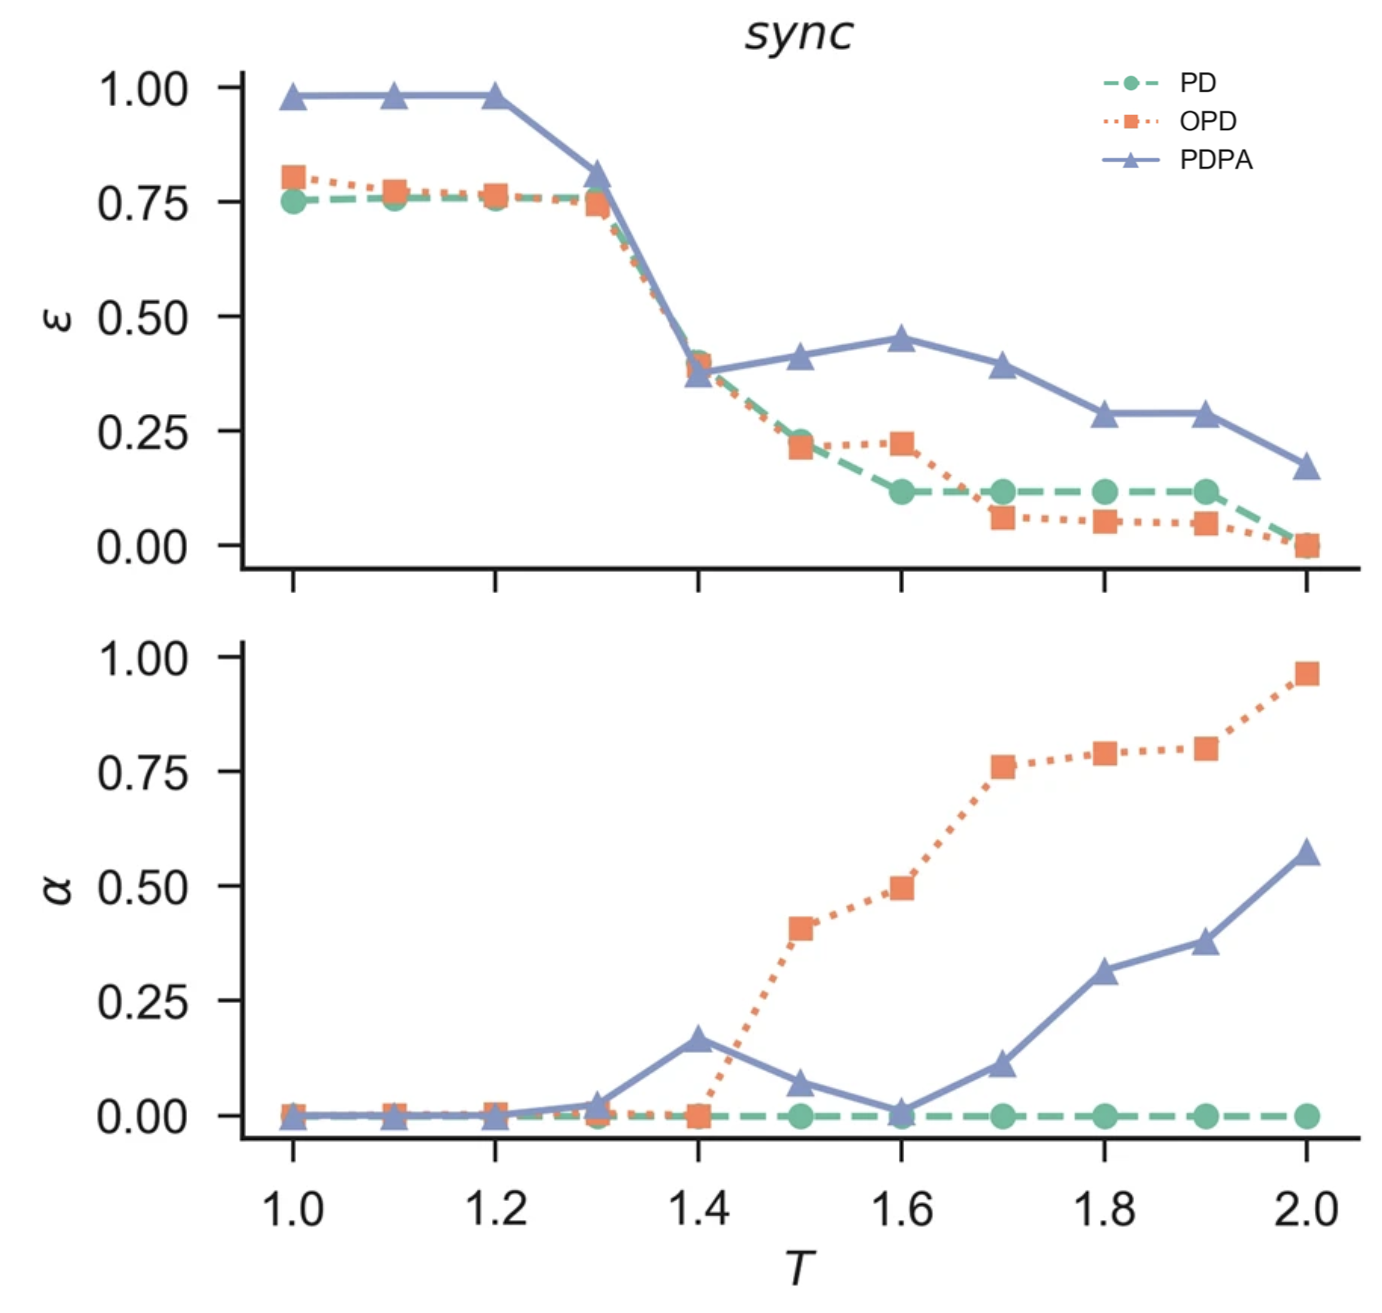
\includegraphics[scale = 0.23]{Images/dependence of alpha and epsilon on T.png}}
    \caption{(a) shows the dependence we obtained for $\alpha$ and $\epsilon$ with respect to $T$ while playing the prisoner's dilemma game, or some variants. Parameters: $R = 1, S = 0, P = 0, L = 0.4, \eta = 0.001$ and $t = 200$. The results are obtained after averaging over 10 runs. (b) corresponds to the results obtained from Cardinot \emph{et al.}  \cite{cardinot2018} using the same values for the parameters.}
    \label{fig: comparison of epsilon and alpha}
\end{figure}

We have chosen to reduce the number of runs and the time for each run compared to the one used in the paper mainly for numerical reasons.

From the grid it was clear that for some values of $T$ there was a correlation between defectors and a high abstention probability $\alpha$ while playing the PDPA game.
We decided then to plot the number of cooperators and defectors for each value of alpha after 200 iterations with $T$ being set equal to $1.4$.
The graph we obtained can be seen in \Cref{fig:correlation}.

This result can be interpreted in the following way:
cooperators tend to organise in clusters in order to survive, they want to be surrounded by other cooperators since a defector would have the best outcome if they were to play against a cooperator.
On the other hand, the strategy of defection works best when the other player is a cooperator, thus defectors tend to stay closer to cooperators.
This explain why cooperators wants to play and to be surrounded by cooperators.
Defectors instead prefer not playing rather than play against another defector.
This is why in \Cref{fig:correlation} we see a high tendency of defectors to abstain from the game.


\begin{figure}
    \centering
    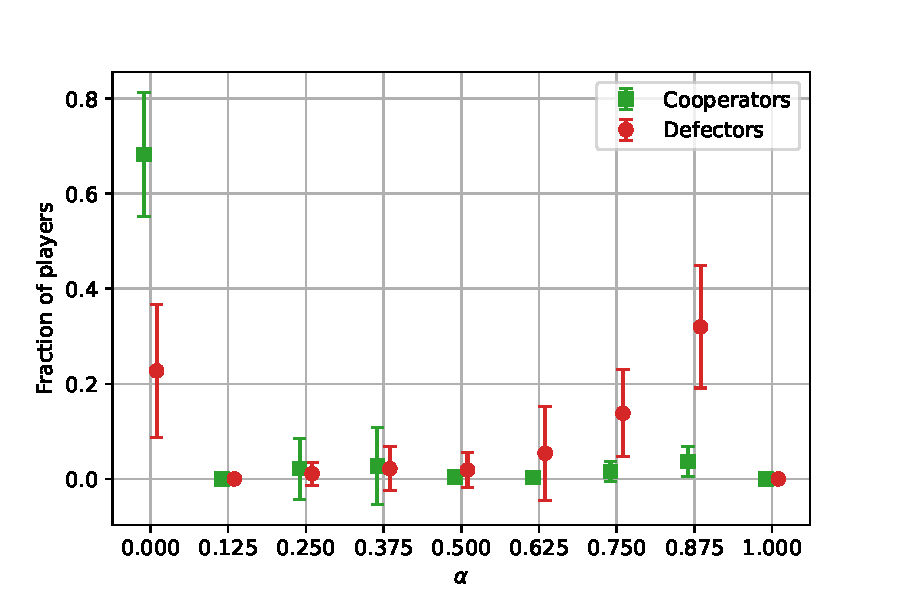
\includegraphics[width = 0.7 \textwidth]{Images/alpha.pdf}
    \caption{Correlation between abstention and cooperation. For each value of $\alpha$, the relative number of cooperators is compared to the relative number of defectors. The numbers are normalized dividing by the total number of players. The marks for cooperators (defectors) are slightly shifted to the left (right) for better readability. Parameters: $T = 1.4, R = 1, S = 0, P = 0.3, L = 0.4$}
    \label{fig:correlation}
\end{figure}

Once we checked that our results are compatible with the ones derived by Cardinot \emph{et al.}, we proceed to analyze the other possible games.
We start by looking at the snowdrift game, as shown in \Cref{fig: epsilon and alpha snodrift}.

\begin{figure}[H]
    \centering
    \includegraphics[scale = 0.7]{alpha_eps snowdrif.pdf}
    \caption{Dependence of $\alpha$ and $\epsilon$ for the snowdrift game on the parameter $T$. In this case we set $R = 1, S = 0.3, P = 0, L = 0.4, \eta = 0.001$ and $t = 200$. The results are obtained by averaging over 10 different runs.}
    \label{fig: epsilon and alpha snodrift}
\end{figure}

In this case we can observe that for $T > 1.4$, the effective cooperation frequency $\varepsilon$ stabilizes.
As long as we keep $T \leq 1.6$, it behaves the same for the three possible cases, and there is no change in the mean abstention probability.

The situation is different when we study the game with $T > 1.6$.
It can be seen that, while the snowdrift game (SD) gives the same results, the optional snowdrift (OSD) and the snowdrift with probabilistic abstention (SDPA) do not.
Both of them show a non-zero expectation value for the mean abstention probability starting from $T > 1.6$ and a decreasing in the effective cooperation. \\
These two effects are more pronounced in the case of the OSD compared to the SDPA.
In fact, since in the OSD the players have either $\alpha = 0$ or $1$ probability to abstain, and since the players can imitate the behaviour of the nearest neighbours, what happens is that the system reaches a steady state because all the players decide to not take part in the game.
Different is the case of the PDPA, where instead some players prefer not to abstain and keep playing, such that the system doesn't actually reach a steady state. 
\begin{figure}[]
    \centering
    \subfloat{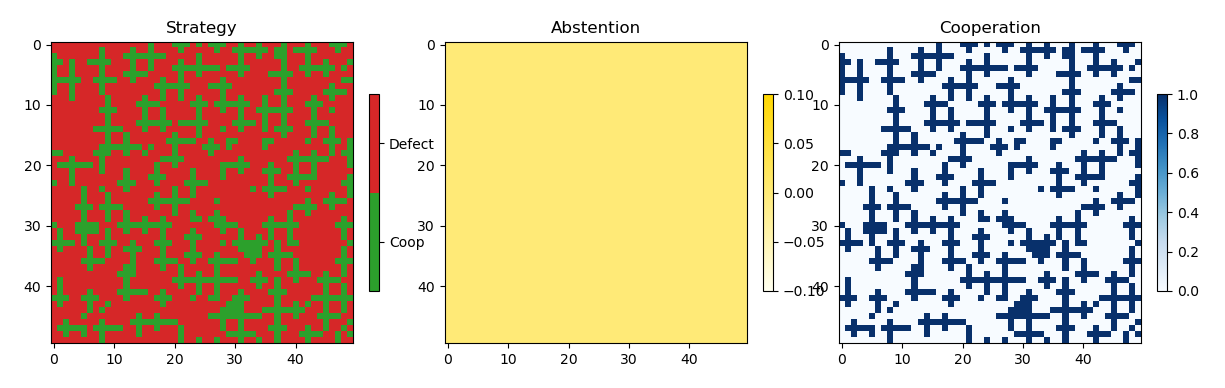
\includegraphics[scale = 0.4]{Images/SD.png}} \\
    \subfloat{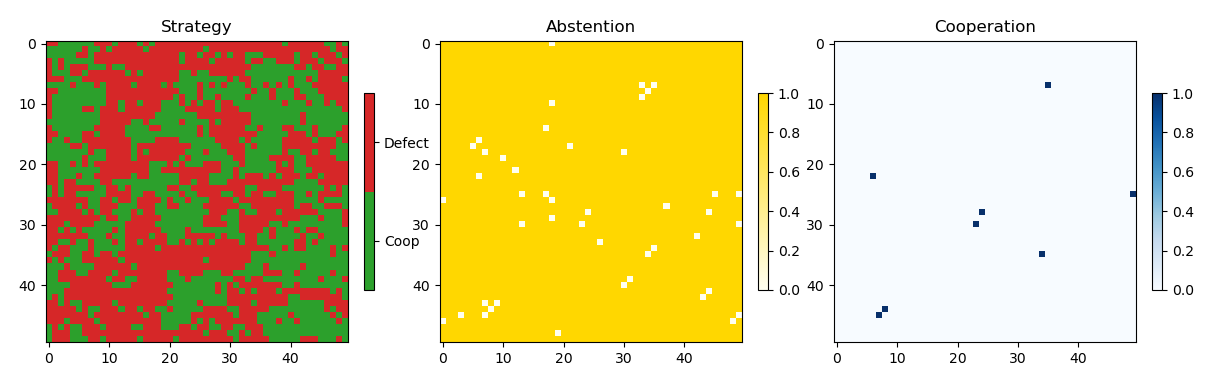
\includegraphics[scale = 0.4]{Images/OSD.png}} \\
    \subfloat{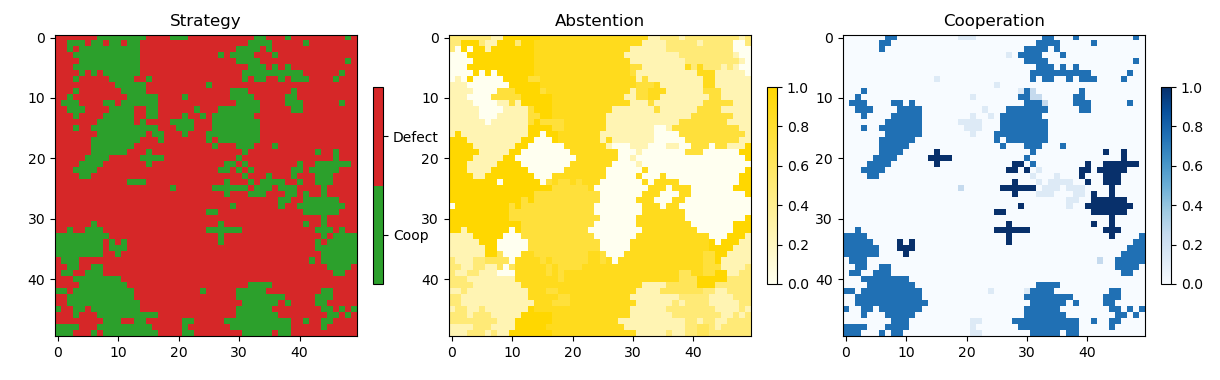
\includegraphics[scale = 0.4]{Images/SDPA.png}} \\
    \caption{Final state of the grid after 200 iterations for three different games (from top to bottom): SD, OSD, SDPA. For each game is shown the final distribution of cooperators and defectors (first column), of the abstention probability $\alpha$ (second column) and of the effective cooperation frequency $\varepsilon$ (last column). All of them have been taken by setting $T = 1.9$. and $\eta = 0.001$}
    \label{fig: screenshots of SD OSD SDPA}
\end{figure}

What is possible to observe in \Cref{fig: screenshots of SD OSD SDPA} is that, as soon as we turn on the possibility for the players to abstain, either in a probabilistic or optional way, we see that the clusters of cooperators increase in size.
The most significant difference between the two is in the fact for OPD we notice a bigger tendency of the players to abstain. 
On the other hand, when the probability of abstention is randomly generated between $[0,1]$, we observe that some players manage to not uniform to the behaviour of the rest and maintain a values different from 1.
There also seems to be a correlation between a low $\alpha$ value and being a cooperator.

We then proceed by studying the remaining two games: the harmony game and stag hunt. 
\begin{figure}[H]
    \centering
    \subfloat[]{\includegraphics[scale = 0.5]{alpha_eps stug hunt.pdf}} 
    \subfloat[]{\includegraphics[scale = 0.5]{alpha_eps harmony game.pdf}}{}
    \caption{(a) show the dependence of $\epsilon$ and $\alpha$ on $T$ in the case of the stag hunt game. In this case the parameters chosen for the game are $R = 2, S = 0, P = 0.3$ and $L = 0.4$. (b) correspond the dependency of $\epsilon$ and $\alpha$ as function of $T$ in the case of the harmony game. In this other game the parameters chosen are $R = 2, S = 0, P = 0.3$ and $L = 0.4$. For both games, the results have been taken as an average over 10 runs by setting $\eta = 0.001$ and $t = 200$.}
    \label{fig: harmony game and stug hunt}
\end{figure}

What the results prove is that there is no significant dependence on the temptation payoff in both games not even when the players are allowed to abstain.
Moreover, the different possible ways that the players have to abstain do not affect the result.
In fact, even though at time zero the players have the possibility to not play, after a certain number of iterations we see that the players converge to the decision of playing rather than abstaining.

\section{Conclusions}
\label{sec:conclusions}
First we have reproduced the results obtained from Cardinot \emph{et al.}, which show how the possibility to abstain from playing the game significantly affects the results in the PD.
We checked that actually there is a correlation between being a defector and having a high abstention probability when playing PDPA with $T = 1.4$.

We have then played these variants with abstention also with other games.
The most interesting results have been obtained in the case of the snowdrift game.
In fact, in this case we have seen that for $T > 1.6$ the system shows a different behaviour because of the presence of abstention and is susceptible on which type of abstention we choose, either optional or probabilistic.\\
This is instead not true for the remaining two games, HG and SH, where the system is not affected by the presence of abstention and the results are equivalent to the one obtained for the simple version of the games.

% Bibliography__________________________________________________________________
% Literature (Additional references can be added to the .bib-file manually, or by using, for example, the free application JabRef). Compile in the following order: latex -bibtex -latex -latex

%\bibliographystyle{plain}
%\begin{footnotesize}
%    \bibliographystyle{apalike}
%    \bibliography{references}
%\end{footnotesize}

\newpage

\printbibliography
\end{document}
